\section{Components}

\begin{itemize}
  \setlength\itemsep{0em}
  \item One game map
  \item 60+ wooden blocks
  \item 33 action cards
  \item 4 dice
  \item This rulebook
\end{itemize}

\subsection{The Game Map}
The map has been divided into areas, with most areas home to one or two specific tribes. The name of each area is the name of the tribe or tribes that inhabit that area and is their home.

The Roman home area is Transalpine Gaul. There is also a Roman off-map area. Both of these areas are red. The German home area is Germania. It represents an amalgam of various German tribes that lived across the Rhine river. Between them is Gaul, which contains the various Gallic tribal areas.

The color groupings used in Gaul are to aid with the setup and represent the historical regions of Gaul - green for Belgica, grey for Celtae and dark green for Aquitaine. The map also contains a key that explains some of its features.

Some areas have a Fortified Town symbol. These areas provide potential bonuses for a defending block, and supply points for the Romans. The border between each area is either black or blue. The blue borders denote rivers or terrain that can limit movement. The Alps and Rhine River incur certain penalties or bonuses.

The ocean between Britannia and Gaul is divided into two sea zones - Oceanus Britannicus and Mare Cantabricum - and is not playable except by amphibious movement. Most coastal areas contain a port symbol. Units that start their action in port space can move amphibiously from their current area to another area within the same sea zone that also contains a port symbol. The Osismi area is the only area connected to both sea zones.

The Turn Track keeps a record of what turn it is. There are eight turns, with each turn representing one year. In addition, it shows the die roll necessary to bring in additional Roman reinforcements (if playing with the historical reinforcement schedule). It can also be used to track whether or not Caesar or Ariovistus wintered for the turn. The Supply, Tribes Controlled and VP markers are used to track their respective factors in the game. Each side side has an area on the map to place cards that were used to activate a neutral tribe to help players remember their respective limits.

\par
\subsection{The Units}
Each unit is represented by a colored block with the appropriate label applied. To apply the labels, peel them from the label sheet and position it in the center of the appropriate colored block for that label. Once positioned, press the label down firmly. Only one label should be applied to each block.

Apply the red (Roman) labels to the black blocks, the blue (German) labels to the blue blocks, the grey (Gallic - Celtae) labels to the grey blocks, the green (Gallic - Belgae) labels to the green blocks, and the dark green (Gallic - Aquitaine) labels to the green blocks.

Each unit has a number on each side that represents its strength, which also represents the number of dice it rolls in battle. Strength numbers are black print. As units take hits in battle they are reduced in strength by rotating the block counter-clockwise.

In the upper right corner of each unit is its Initiative Rating that determines the order in which a unit performs battle. There are three possible initiative ratings - A, B, C, D. Units with an 'A' initiative perform battle first, then 'B' units, then 'C' units, and finally 'D' units.

In the lower right corner of each unit is its Battle Rating, which is the numeric value needed or less on a 1d6 die roll to score a hit when performing battle.

Each unit also contains its name. For Roman legions, a Roman numeral indicating the legion number. For Gallic and German units, the name of the tribe. Gallic units may also include their tribal home area on the bottom (for German units the tribal name is purely for flavor, Germania is the home of all German units). For leader units, the name of the leader is printed on the block. The movement rate for all units is one area. Note that in some cases, different Gallic tribes share the same home area.

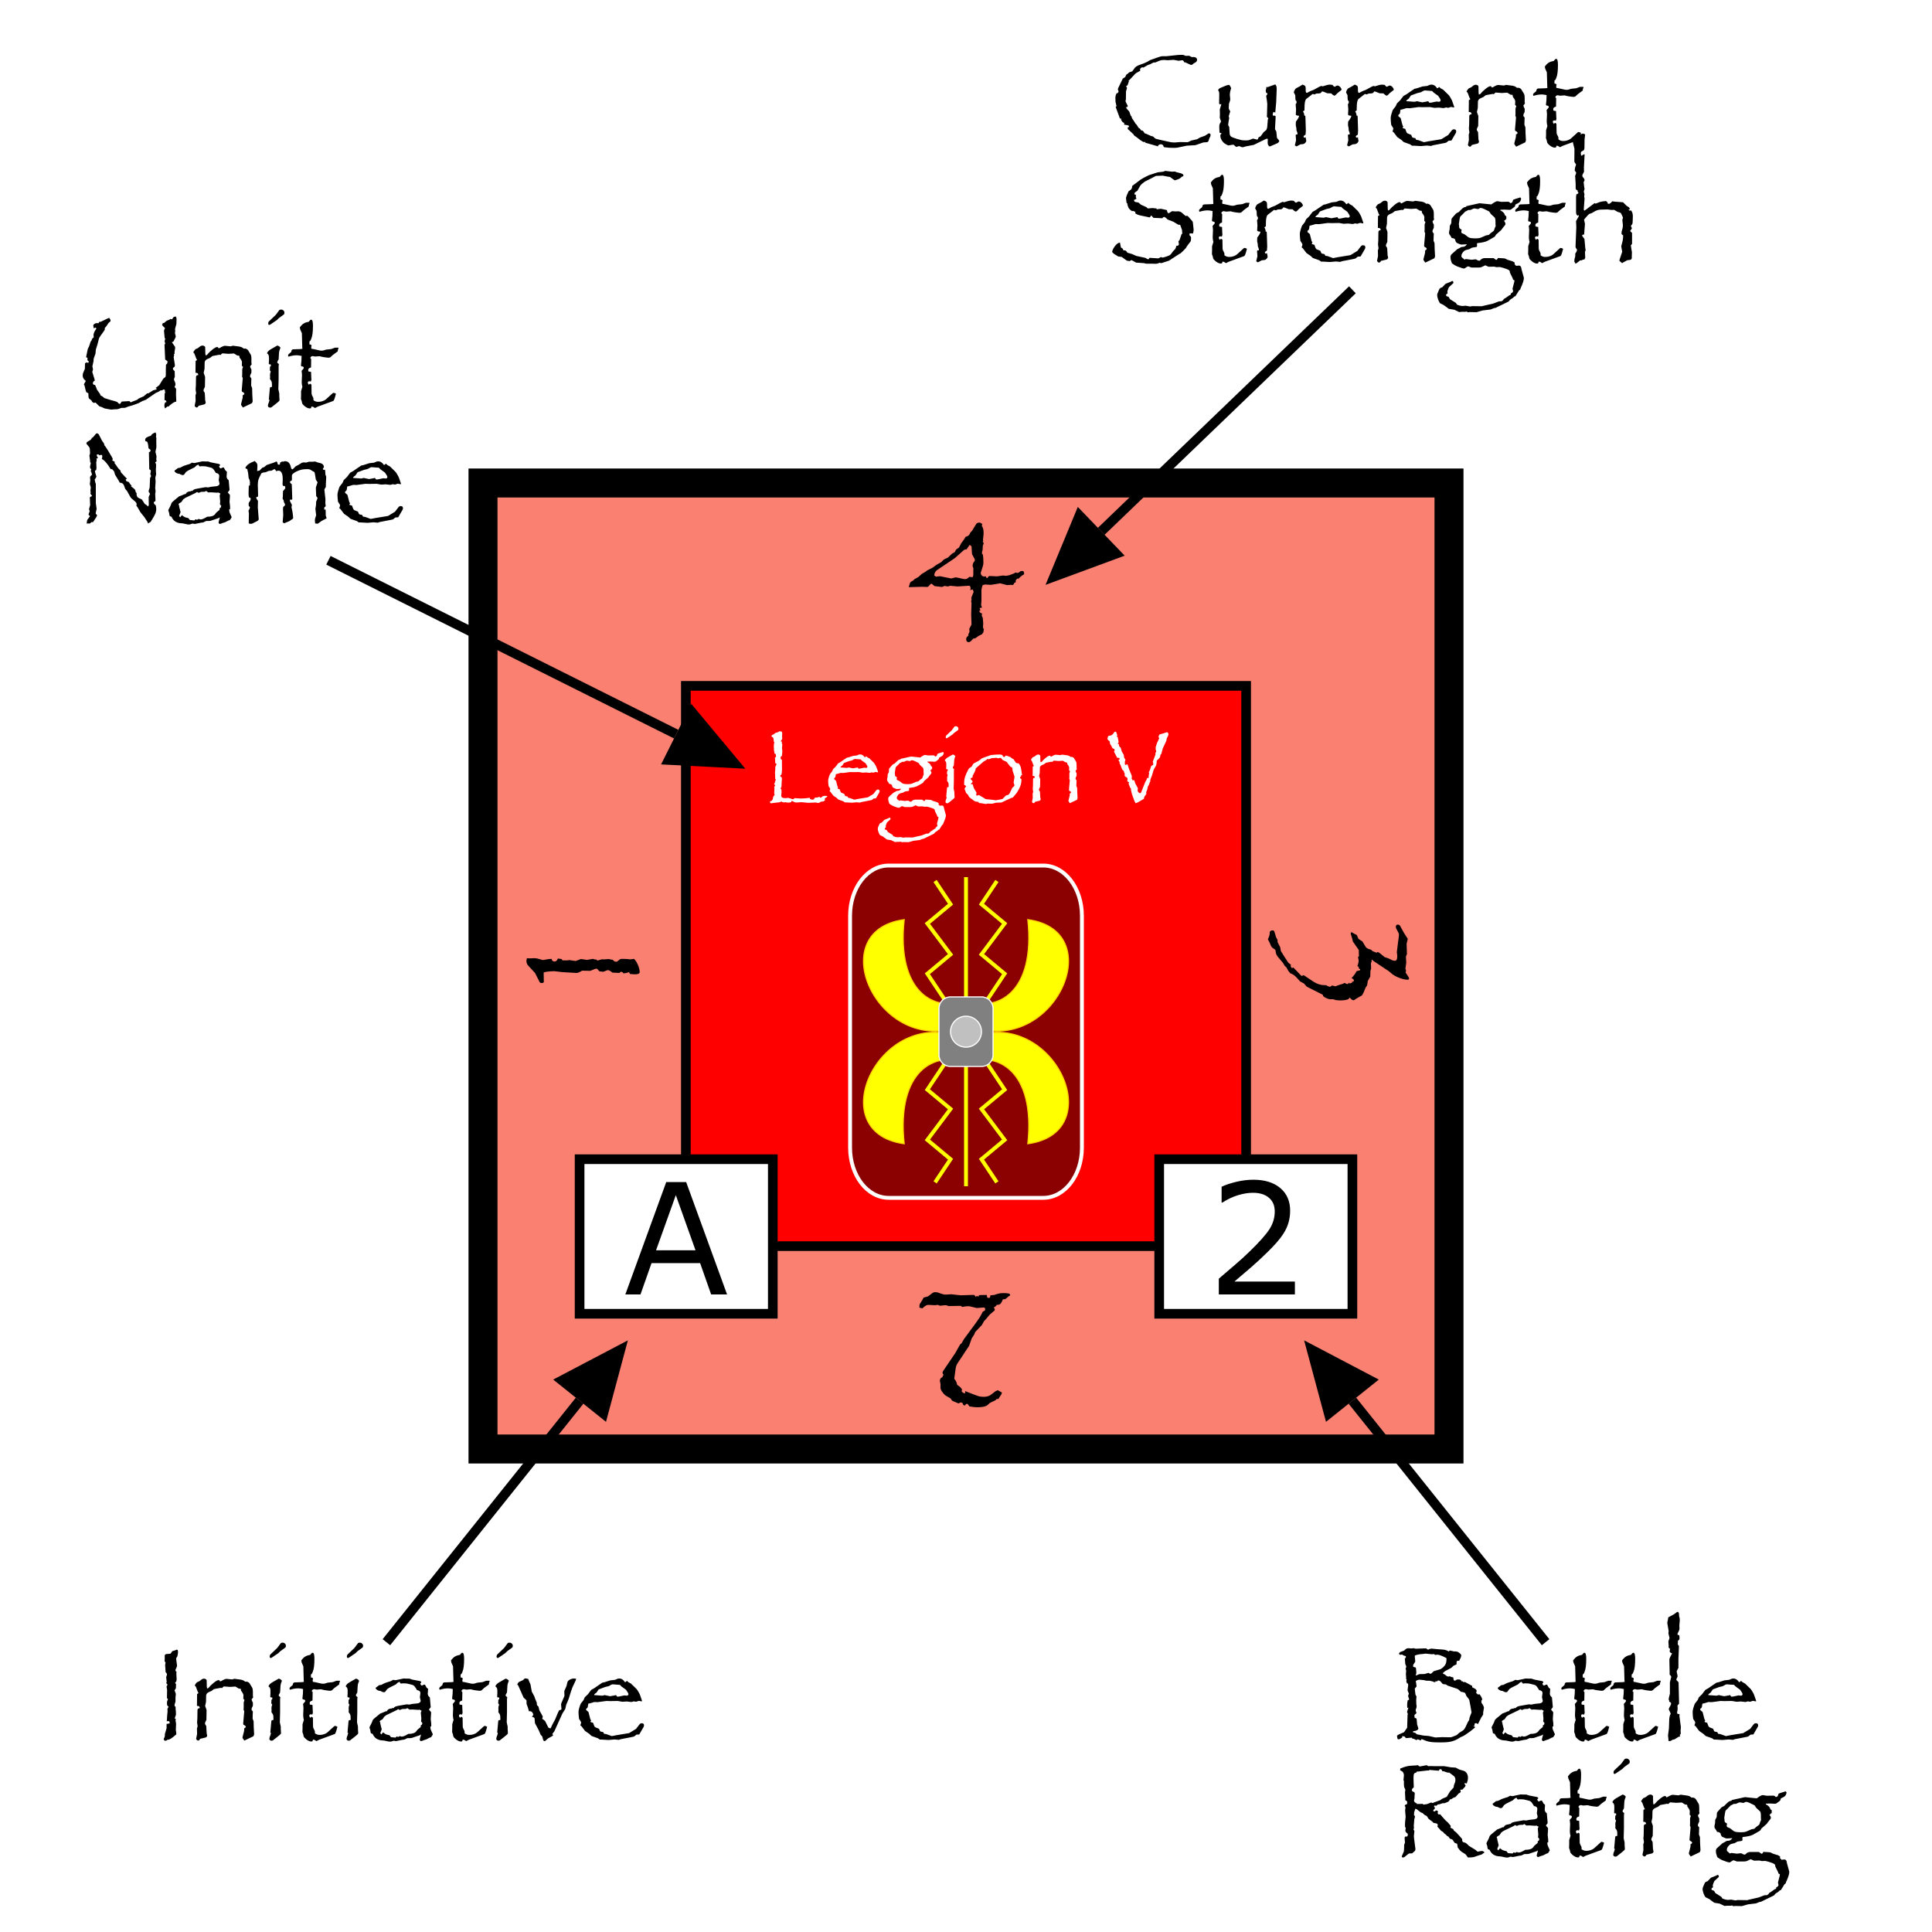
\includegraphics[width=0.45\linewidth]{Unit_Description.png}
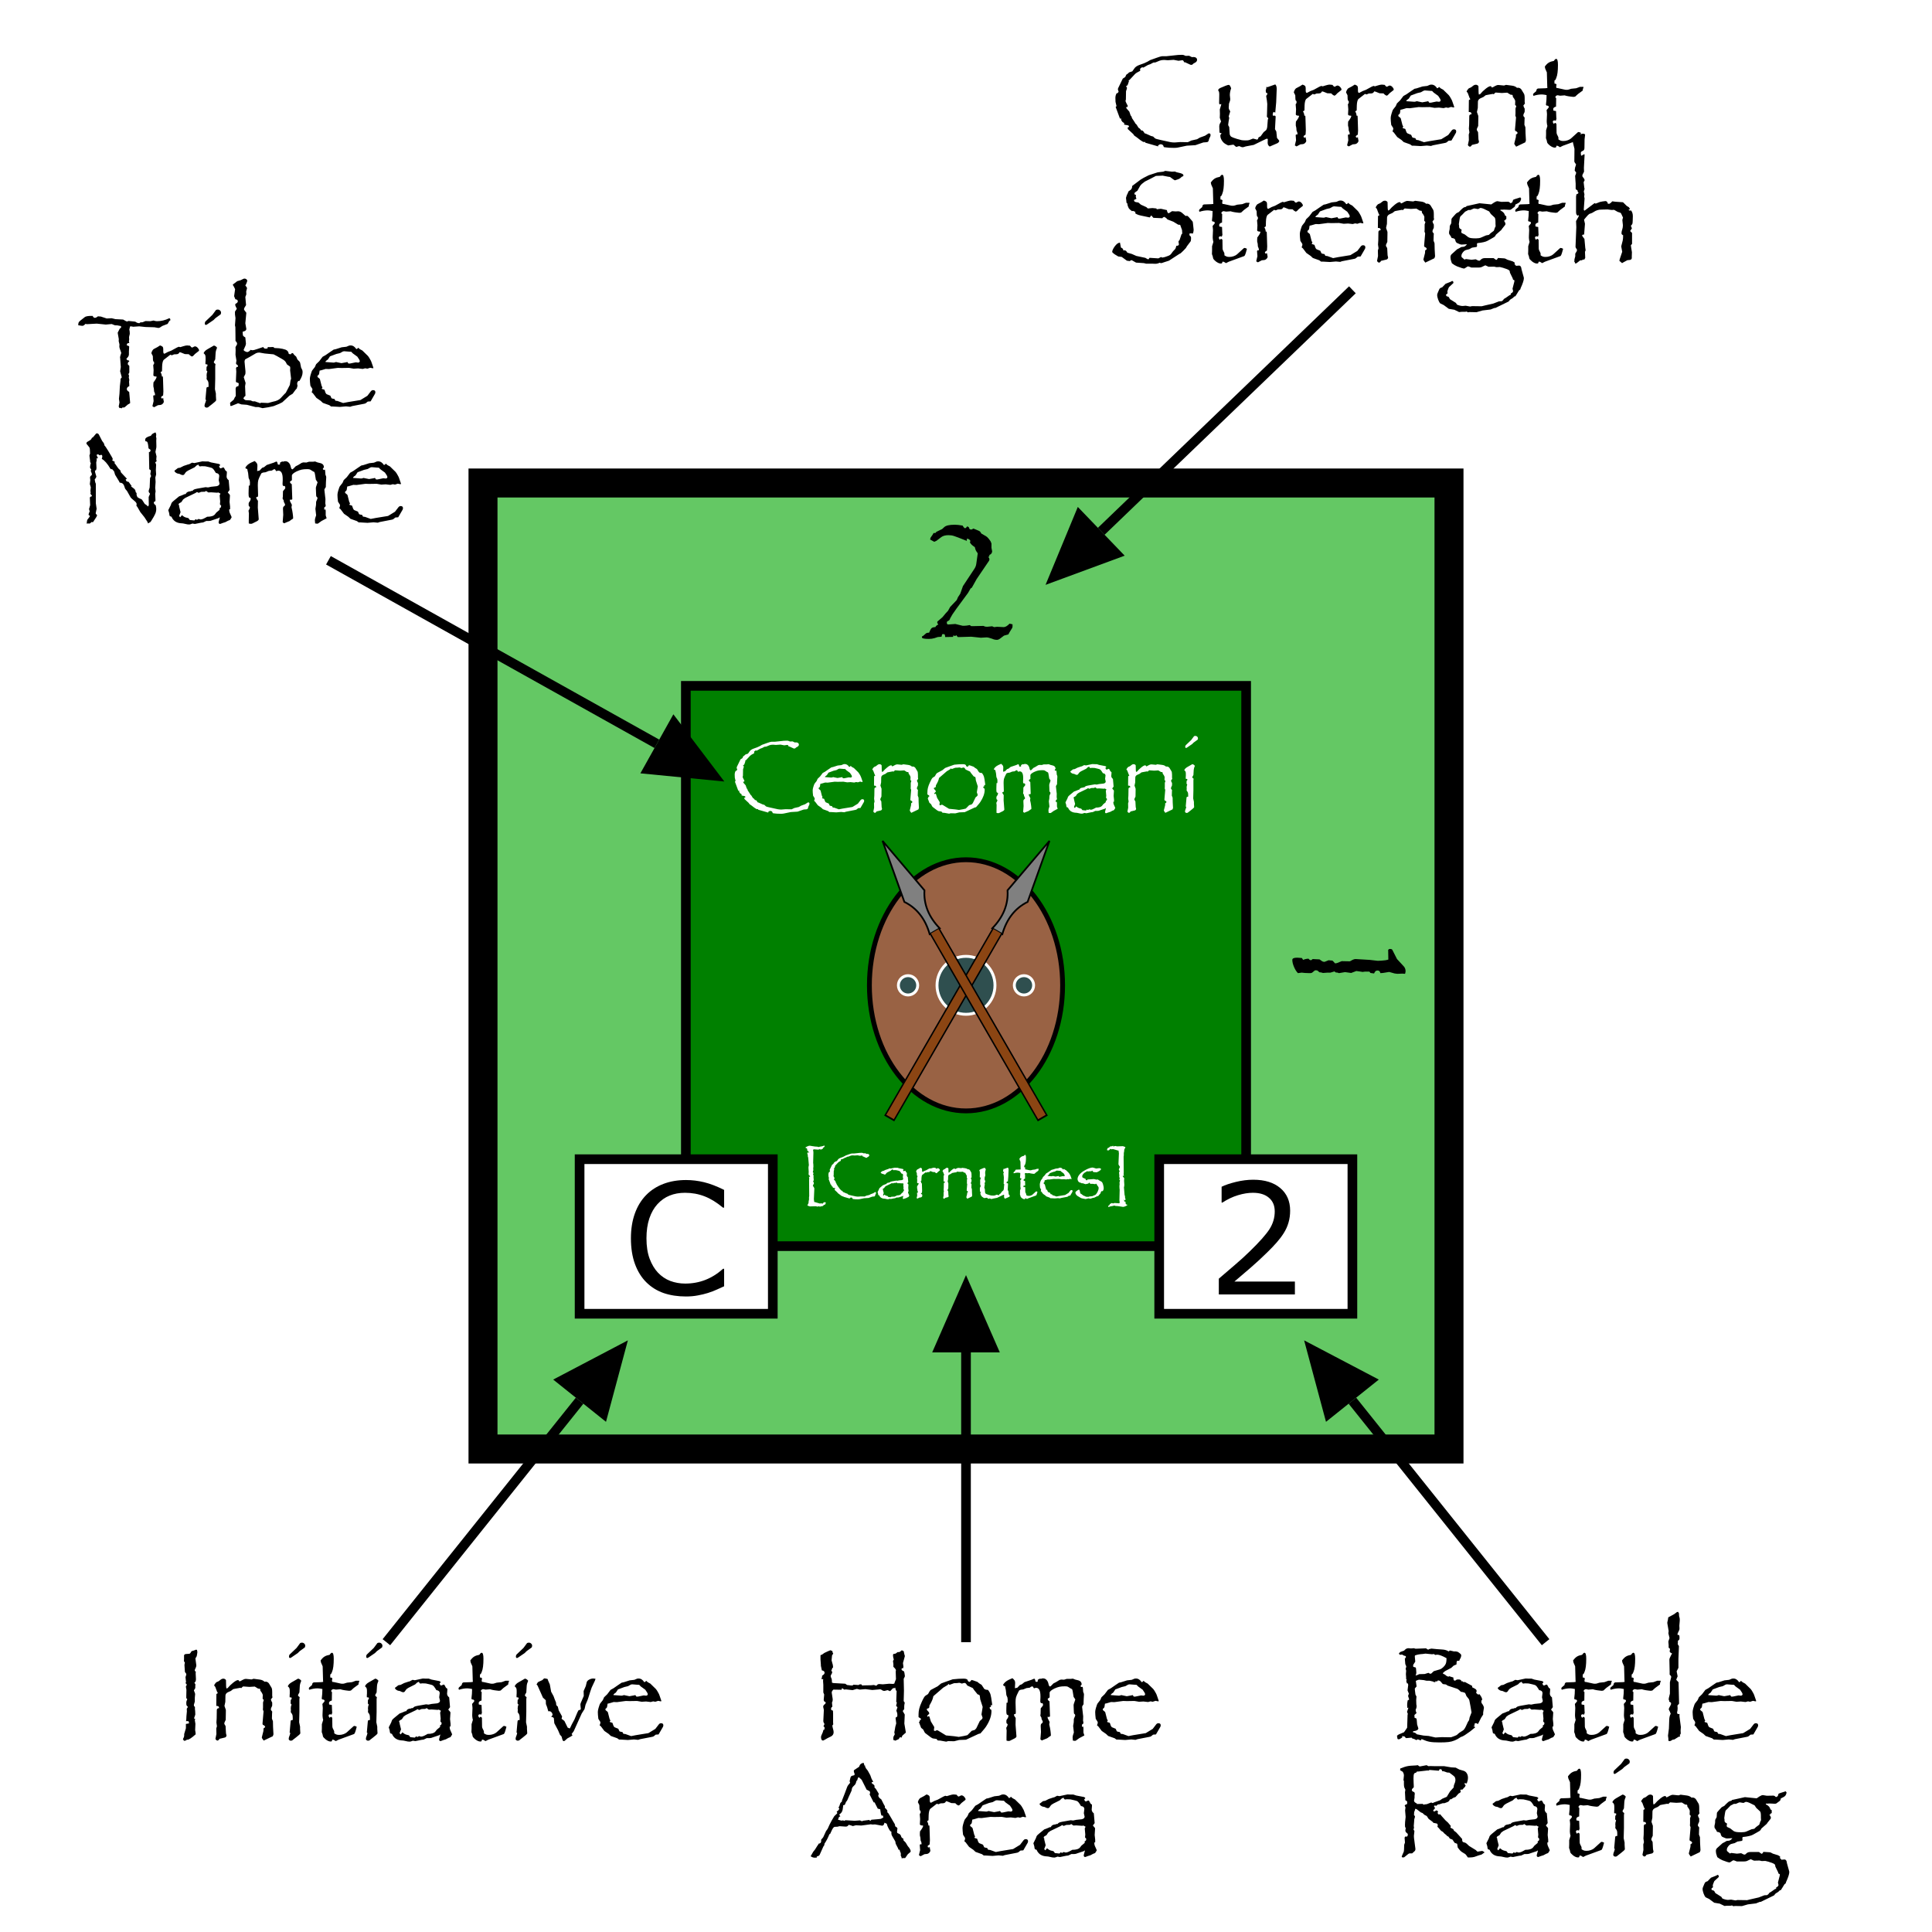
\includegraphics[width=0.45\linewidth]{Barbarian_Unit_Description.png}

The black Roman blocks are controlled by the Roman player. The blue German blocks and the grey and green Gallic blocks start the game neutral and are controlled by neither player. They are placed face-down on the board, while units controlled by a player are placed face-up with the label facing the controlling player. Players may not look at their opponent's unit labels.

Active Gallic tribes controlled by the Roman player are considered Roman allies. Active Gallic tribes controlled by the Barbarian player are considered Barbarian allies. The phrase "Roman units" refers to both Roman units and Gallic tribes that are Roman units, while "Roman legion" refers specifically to the black Roman blocks. The phrase "Barbarian units" refers to both German and Gallic tribes that are allied to the Barbarian player. The phrase "Germanic units" refers only to the blue German blocks.

\begin{figure}[h]
  \centering
  \begin{minipage}{0.19\linewidth}
    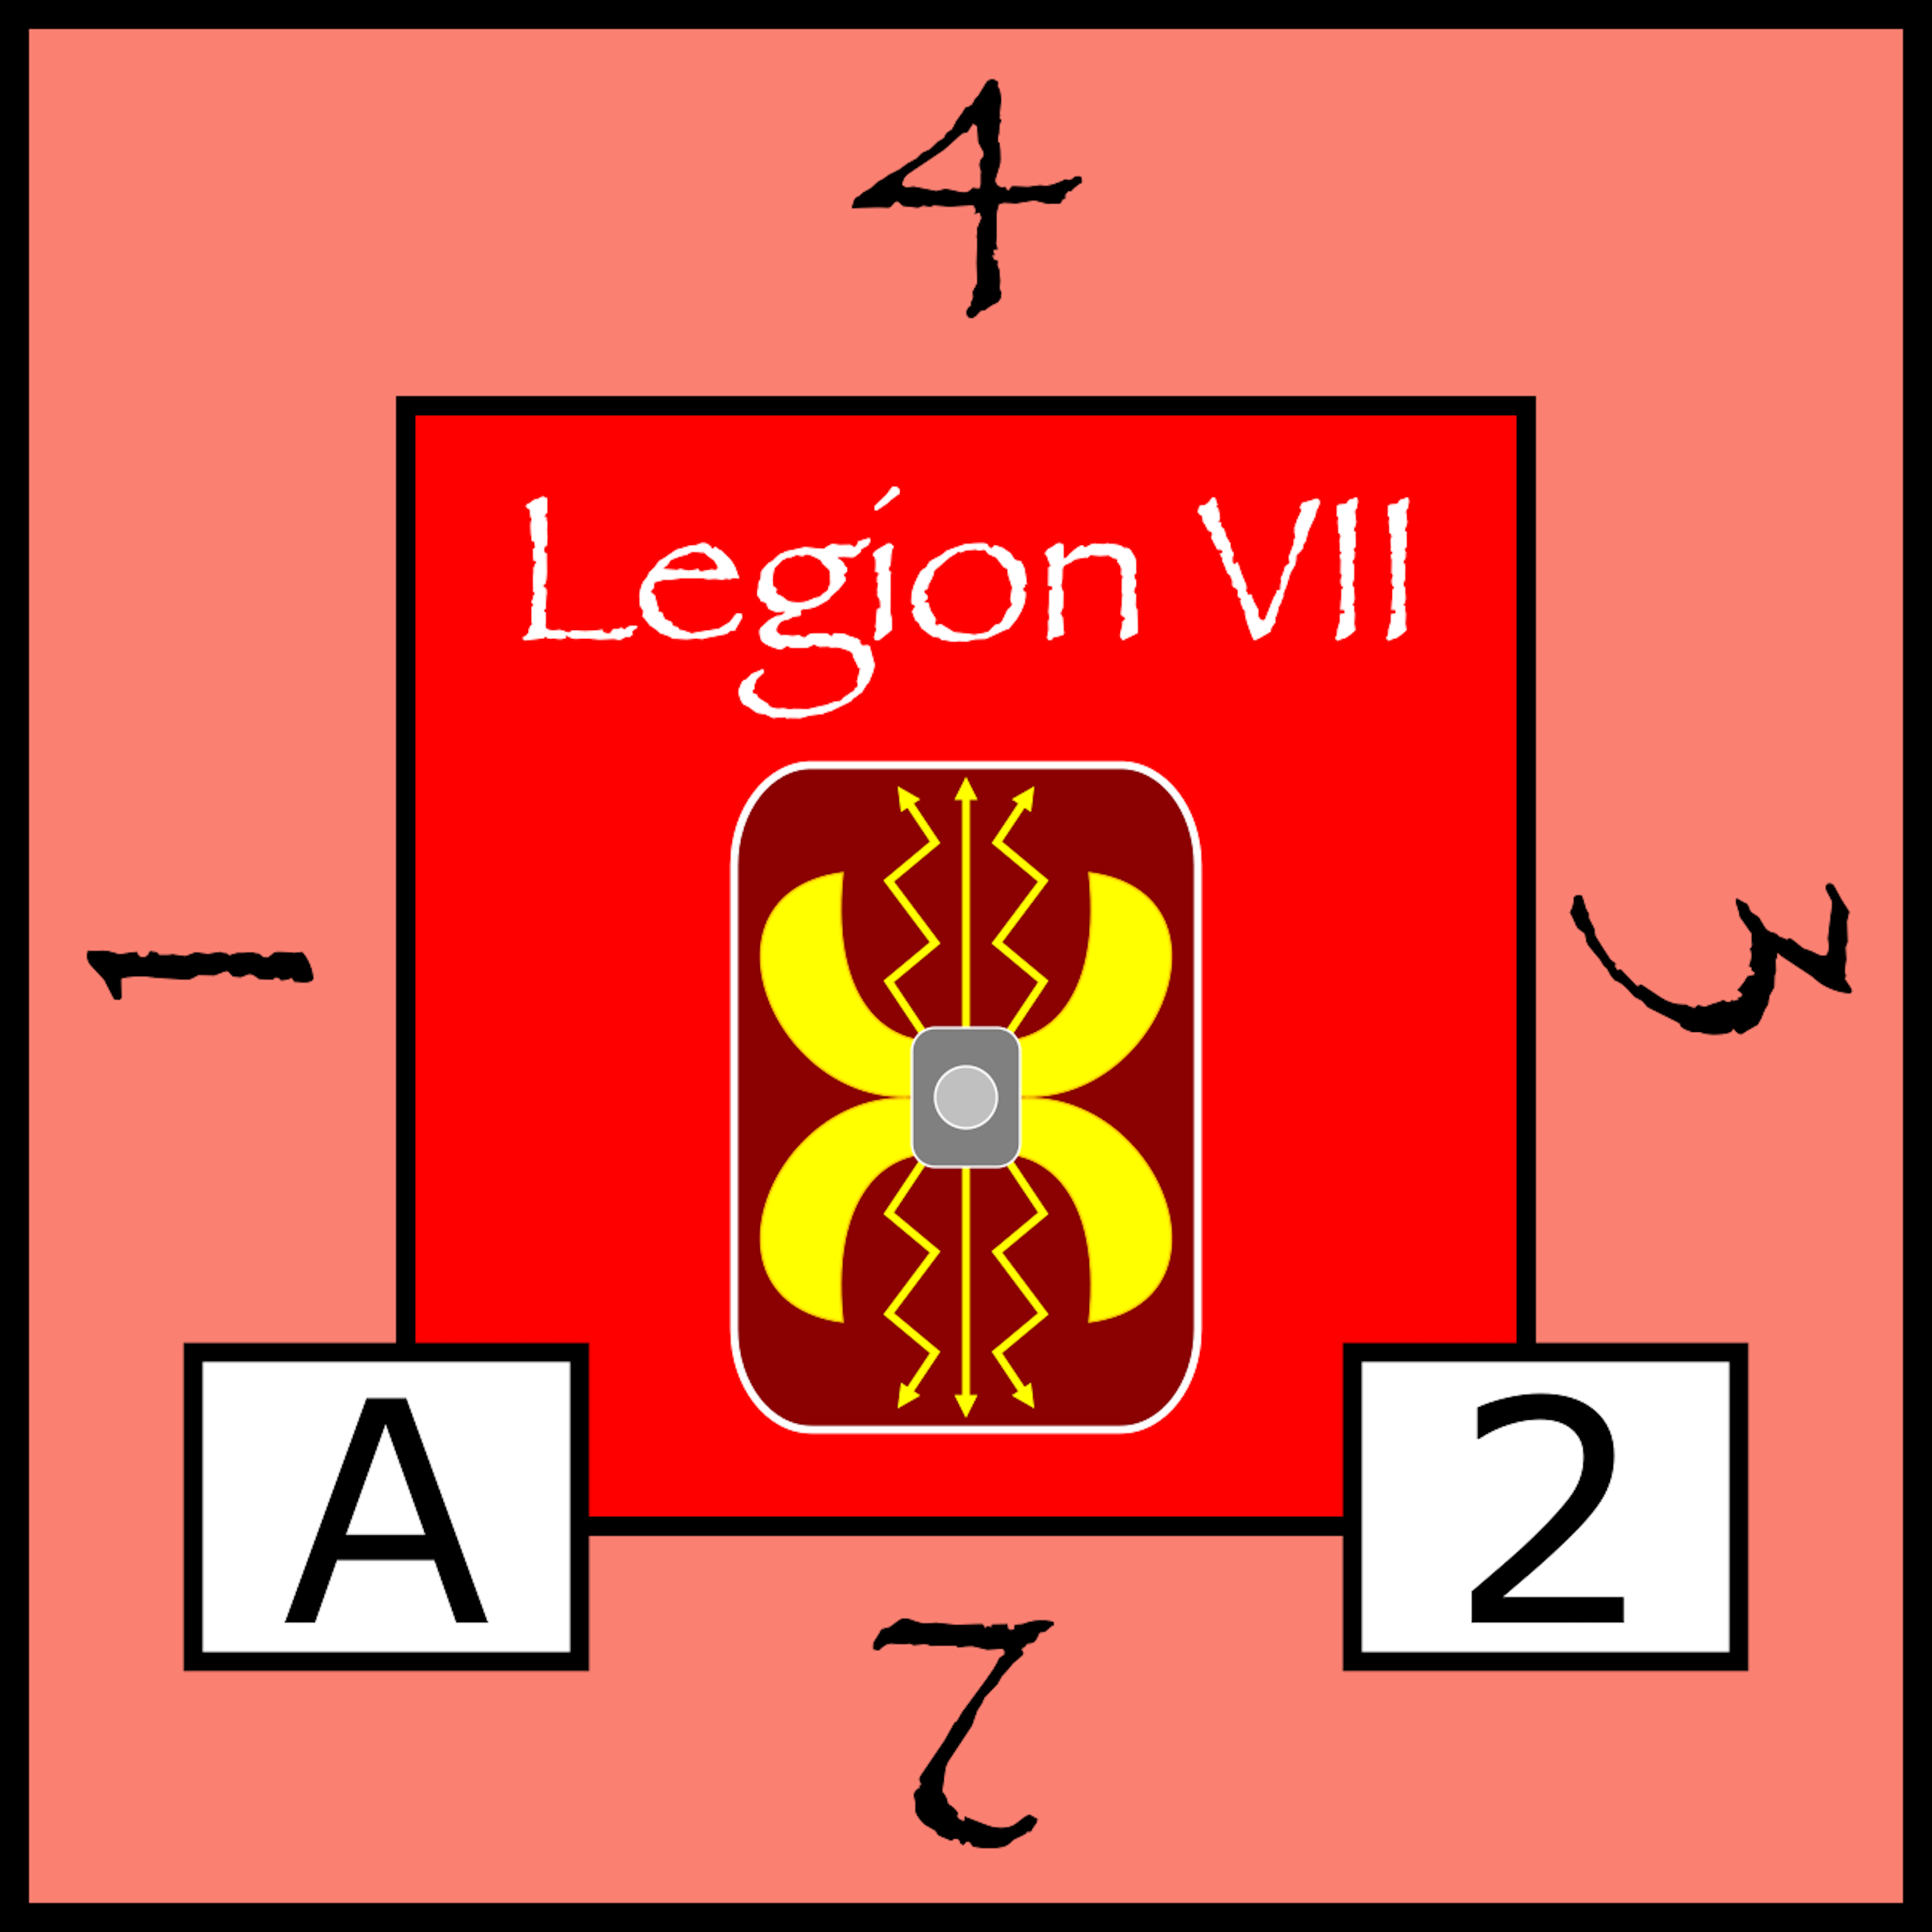
\includegraphics[width=\linewidth]{Legion_VII.png}
    \centering Roman
  \end{minipage}
  \begin{minipage}{0.19\linewidth}
    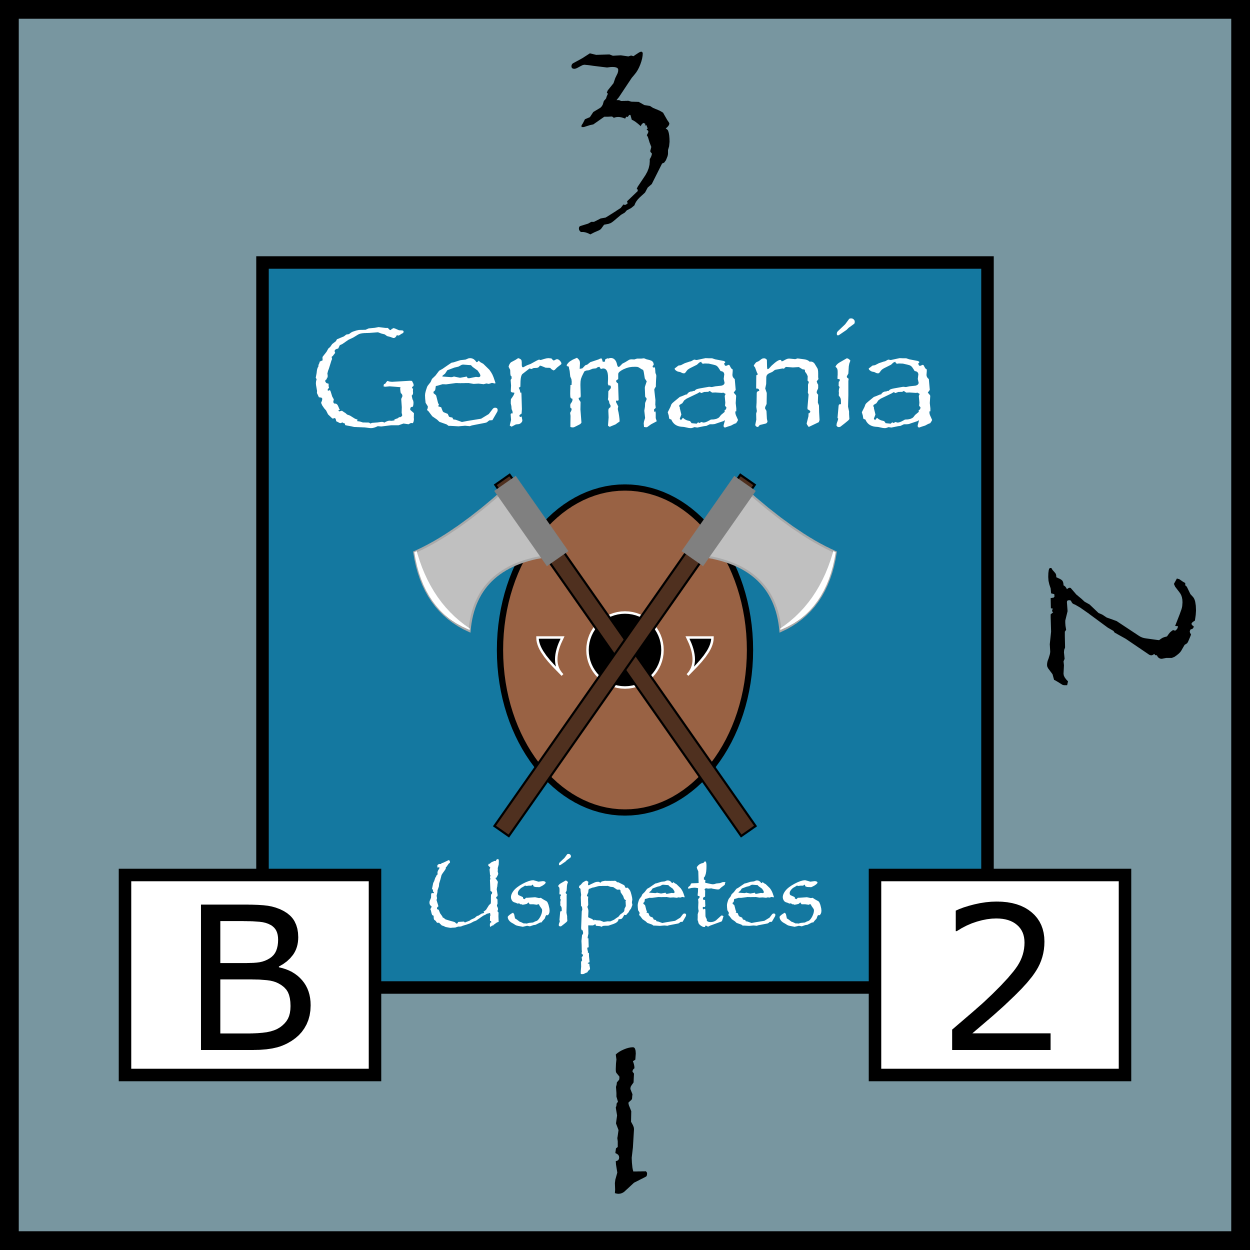
\includegraphics[width=\linewidth]{German_Usipetes.png}
    \centering German
  \end{minipage}
  \begin{minipage}{0.19\linewidth}
    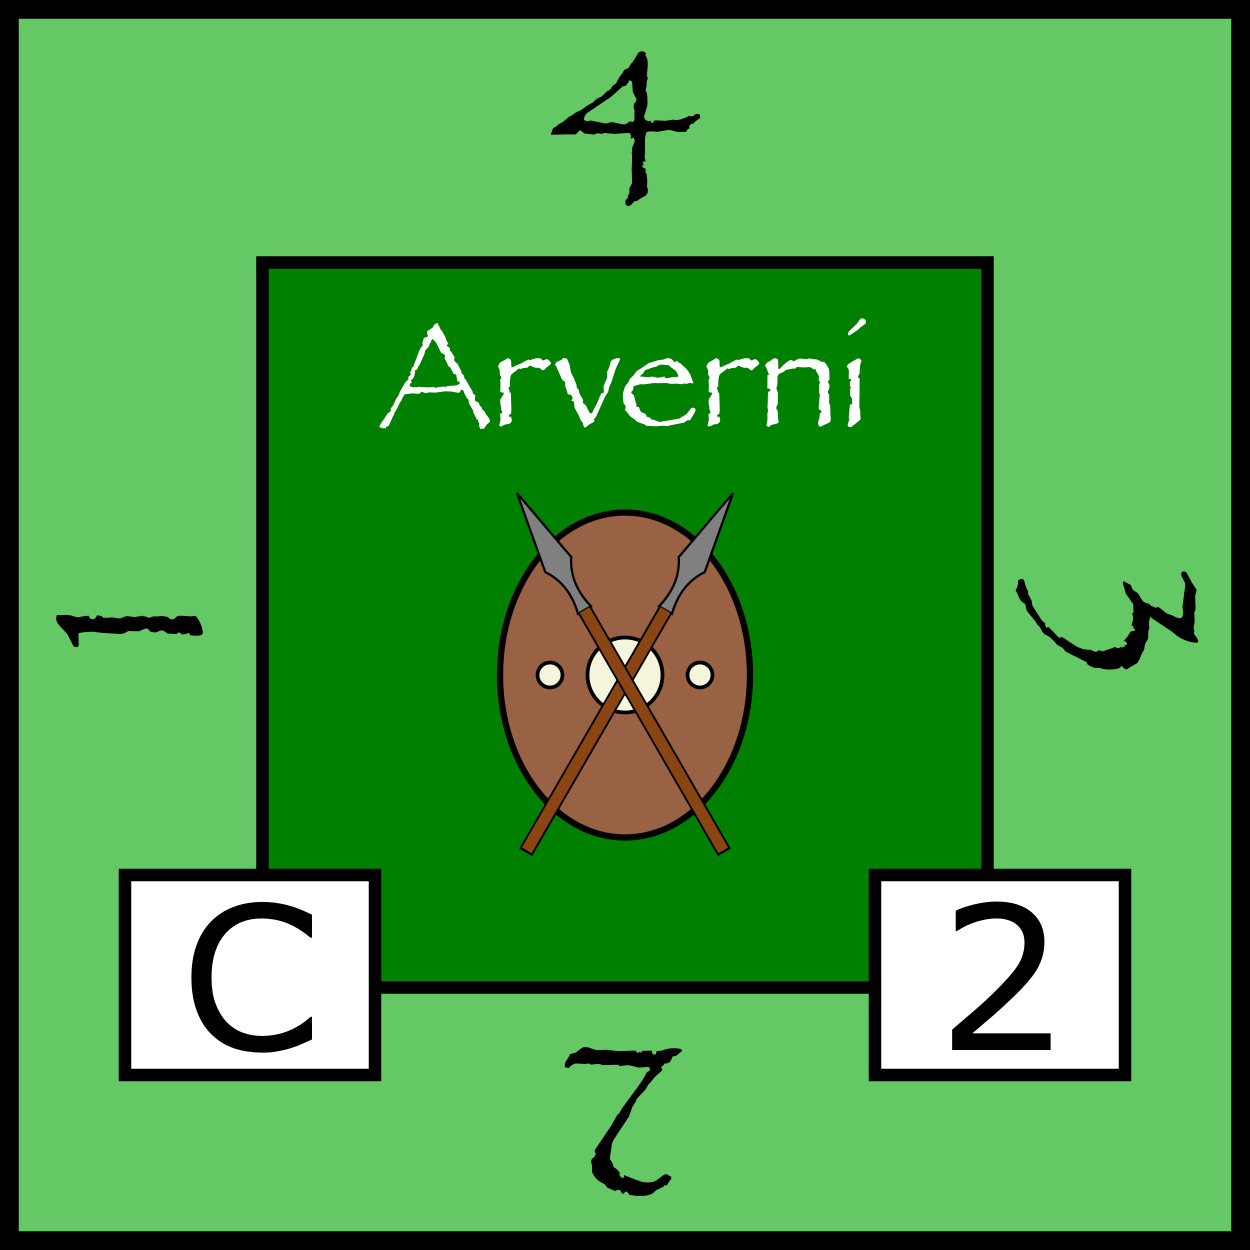
\includegraphics[width=\linewidth]{Arverni.png}
    \centering Celtae
  \end{minipage}
  \begin{minipage}{0.19\linewidth}
    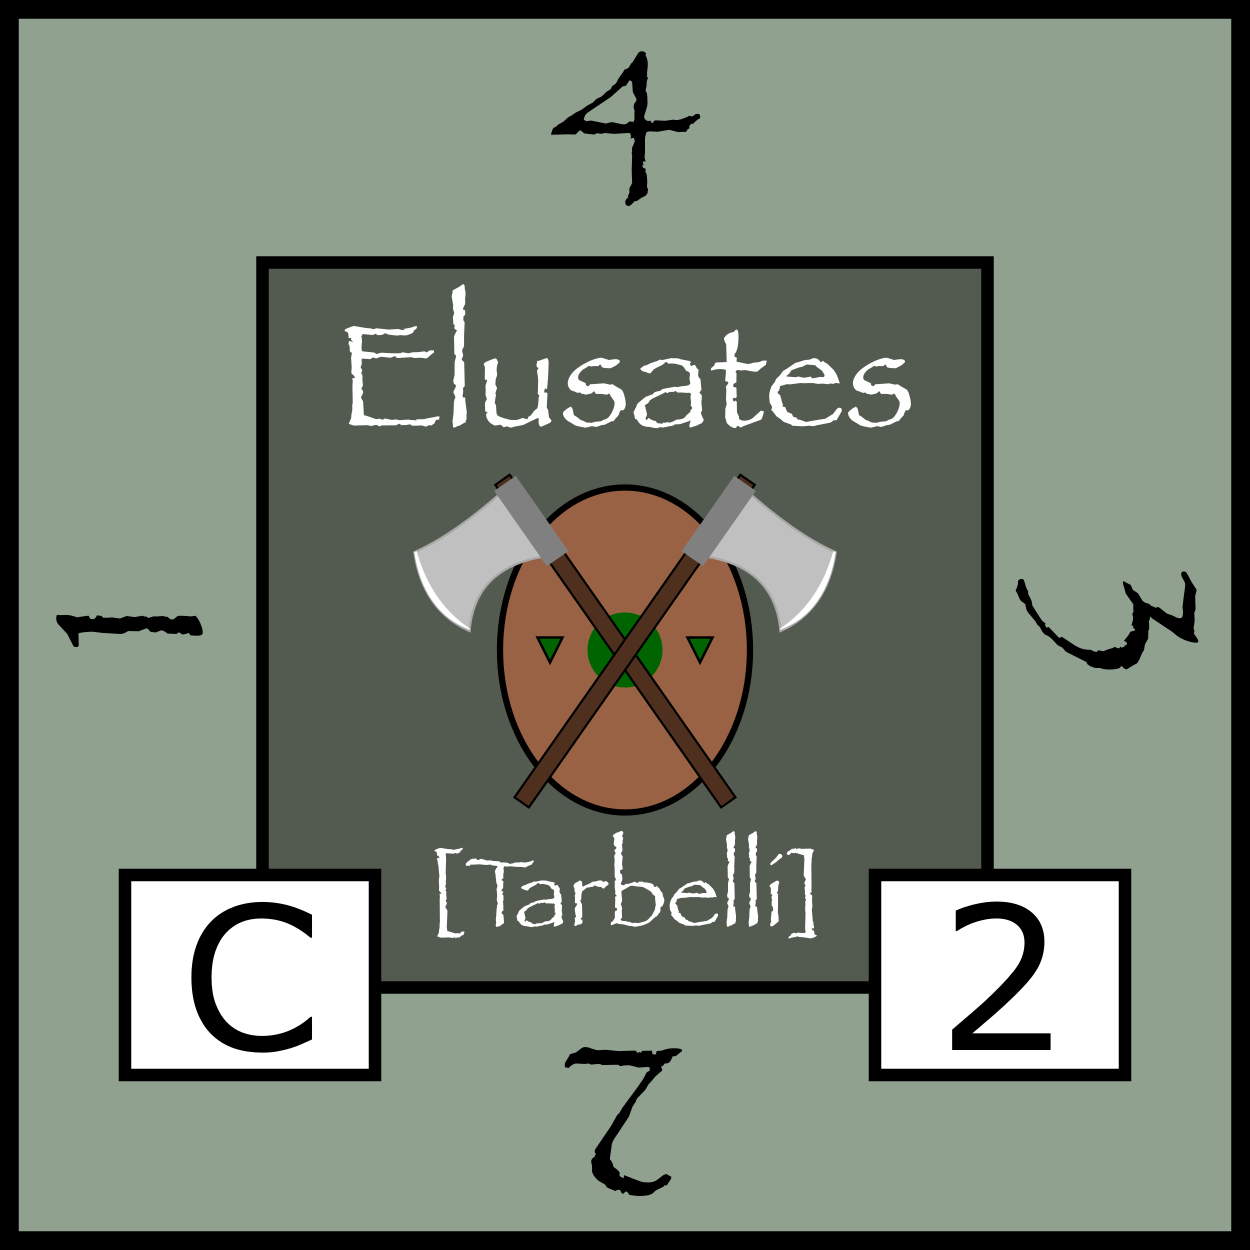
\includegraphics[width=\linewidth]{Elusates.png}
    \centering Aquitani
  \end{minipage}
  \begin{minipage}{0.19\linewidth}
    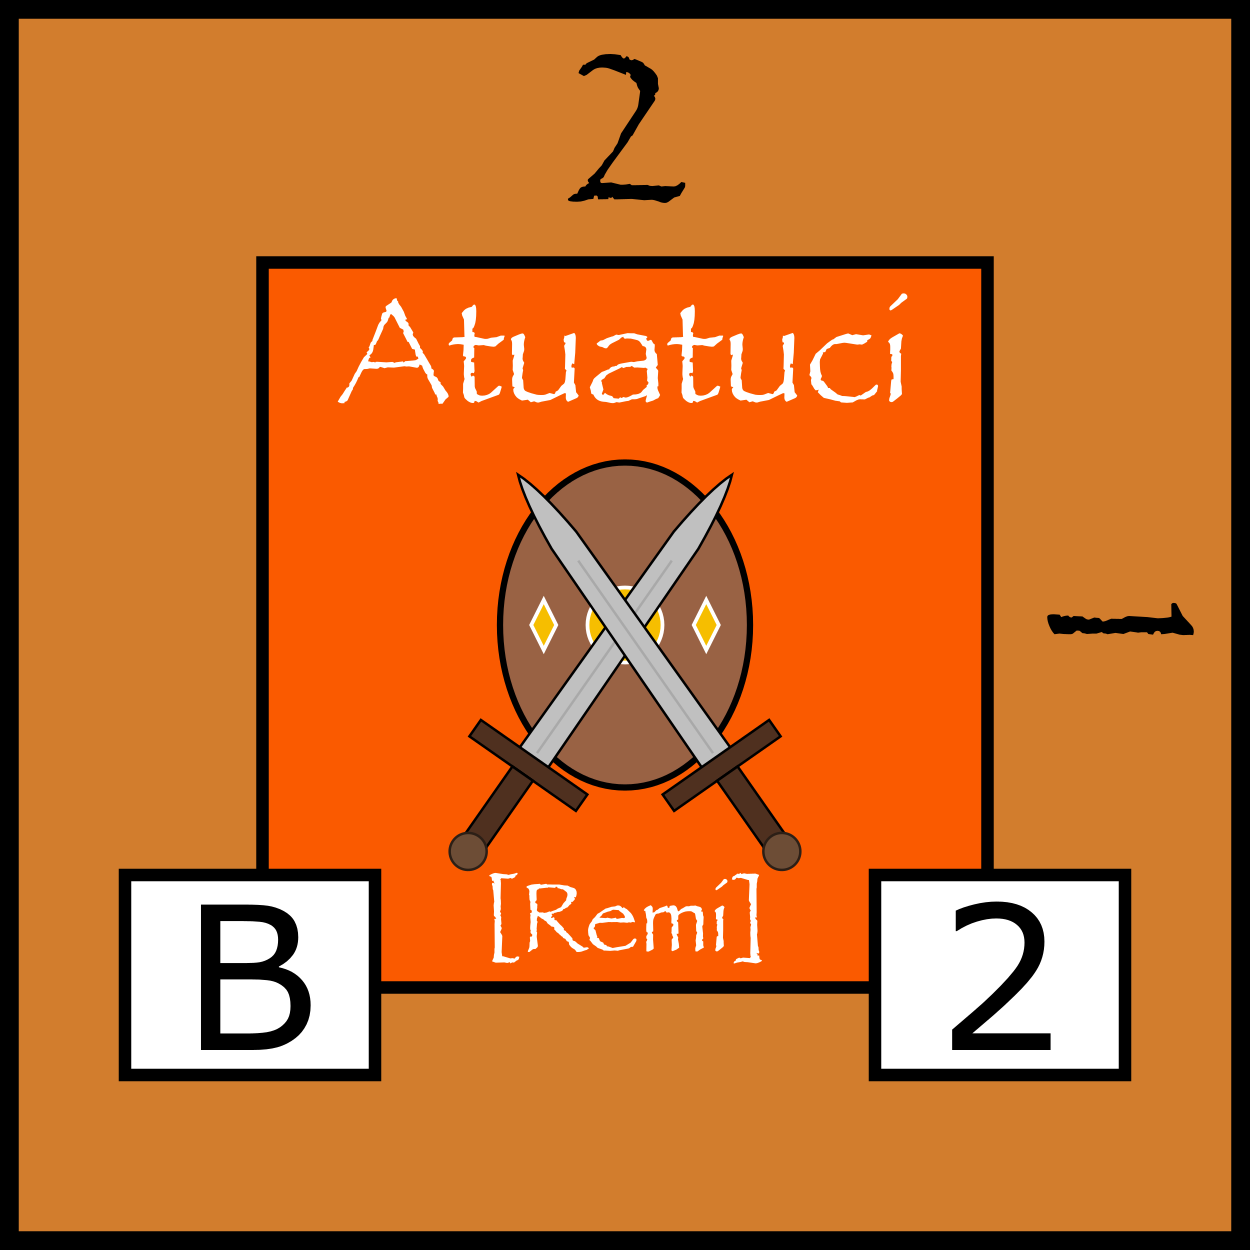
\includegraphics[width=\linewidth]{Atuatuci.png}
    \centering Belgae
  \end{minipage}
\end{figure}

\par
\subsection{The Cards}
Cards contain either the name of one or two Barbarian Tribes with an image of their home area on the card, or an event which summarizes the effect of the event. The Action Point value is printed on the card. Note that in one area - Germania - the Action Point value depends on who plays it. It's "2" for the Roman player, but "3" for the Barbarian player.
